
\documentclass[12pt]{cspcccsthesis}
% preamble
\usepackage{indentfirst}

\title{Beyond LLMs: A RAG Chatbot for Efficient Literature Search and Thesis Retrieval in CSPC Library}
\authorOne{Divino Franco R. Aurellano}
\authorTwo{Herald Carl N. Avila}
\authorThree{Almira L. Calingacion}
\degree{Bachelor of Science in Computer Science}
\approvaldate{January 1, 2020}
\school{College of Computer Studies}
\adviser{Rosel O. Onesa, MIT.}
\dean{Rosel O. Onesa, MIT}
\committeeMemberOne{Kaela Marie N. Fortuno, M}
\committeeMemberTwo{Tiffany Lyn O. Pandes, MSc}
\committeeChair{Joseph Jessie S. Oñate, MSc}
\department{}
\thesisAbstract{Lorem ipsum dolor sit amet, consectetur adipiscing elit. Nunc scelerisque hendrerit fringilla. Vestibulum nec nibh nisi. Curabitur iaculis est lorem, vehicula consectetur erat ullamcorper eget. Aliquam cursus mollis pretium. Fusce bibendum ornare nisl quis dictum. Curabitur tincidunt euismod erat, fringilla elementum ex blandit in. Nunc pretium libero non bibendum egestas. Interdum et malesuada fames ac ante ipsum primis in faucibus. Etiam vitae porttitor eros. Suspendisse pretium feugiat dui, sed posuere erat porta eu. Lorem ipsum dolor sit amet, consectetur adipiscing elit. Nunc scelerisque hendrerit fringilla. Vestibulum nec nibh nisi. Curabitur iaculis est lorem, vehicula consectetur erat ullamcorper eget. Aliquam cursus mollis pretium. Fusce bibendum ornare nisl quis dictum. Curabitur tincidunt euismod erat, fringilla elementum ex blandit in. Nunc pretium libero non bibendum egestas. Interdum et malesuada fames ac ante ipsum primis in faucibus. Etiam vitae porttitor eros. Suspendisse pretium feugiat dui, sed posuere erat porta eu}
\keywords{amet, consectetur, adipisci velit}

% document body
\begin{document}

\makeTitlePage{May}{2025}

% \begin{frontmatter}
%     
% In \begin{approvalPage}{N}, the parameter N is the number of members in the committee. If this is less than 4, the layout of the page is single-column rather than two-column, so change the value accordingly.

\begin{approvalPage}{3}

% Add people in the following format:
% \committeeMember{Member Name}{Member Department/Position}{Member Affiliation}

\end{approvalPage}
%     \makePanelofExaminers{90}
%     \makeDedication{Ad Majorem Dei Gloriam}
%     
\begin{acknowledgments}

I would like to thank the members of my thesis committee for their help in preparation of this work -- Niles Caulder, without whom I would have been doomed to never complete it, Kimiyo Hoshi, who helped to shed new light on many of my ideas, Pamela Isley, with whom I often disagree but who inspires me to be better, Raymond Palmer, who had no small part to play in the formation of the idea, and Kent Nelson, who always had golden advice.

Special thanks are due to the friends and colleagues who made this work possible. Jimmy Olsen and Pete Ross were invaluable both as friends and as sounding boards for some of my more outlandish ideas. Jack Knight, who I met only briefly, was a major influence, and I'm glad we were able to help each other. 

The author gratefully acknowledges the support for this work offered by S.T.A.R. Laboratories under grant award number 3X29YZ4A, and by the Theodore S. Kord Fellowship. Any views and conclusions contained herein are those of the author, and do not necessarily represent the official positions, express or implied, of the funders.

\end{acknowledgments}

%     \makeAbstract
%     \makeTOC
%     \makeListOfTables
%     \makeListOfFigures
%     %
\newacronym{gps}{GPS}{Global Positioning System}
\newacronym{ar}{AR}{Augmented Reality}
\newacronym{ai}{AI}{Artificial Intelligence}
\newacronym{tip}{T.I.P.}{Technological Institute of the Philippines}
\newacronym{dmmmsu}{DMMMSU}{Don Mariano Marcos Memorial State University}
\newacronym{cspc}{CSPC}{Camarines Sur Polytechnic Colleges}
\newacronym{cnn}{CNN}{Convolutional Neural Networks}
\newacronym{lstm}{LSTM}{Long Short-Term Memory}
\newacronym{ml}{ML}{Machine Learning}
\newacronym{cv}{CV}{Computer Vision}
\newacronym{rnn}{RNN}{Recurrent Neural Networks}
\newacronym{svm}{SVM}{Support Vector Machines}

% \makeListOfAcronyms
% \end{frontmatter}

\begin{thesisbody}
    
\chapter{Introduction}
\begin{refsection}

\hspace{1cm}This chapter provides an overview of the study, covering the challenges of the campus library, the study’s objectives, and its significance. It defines the problem, outlines research goals, and highlights the proposed system’s potential impact. The scope and limitations clarify its boundaries, while the project dictionary and notes offer essential terms and supporting details. 

\section{Background of the Problem}

\hspace{1cm}Large Language Models (LLMs) such as OpenAI's ChatGPT \cite{achiam2023gpt}  and Deepseek \cite{guo2025deepseek} have made significant advancements in Natural Language Processing (NLP) by excelling in diverse applications such as conversational chatbots, text summarization \cite{lewis2019bart}, and code summarization and generation \cite{nijkamp2022codegen,chen2021evaluating}
 In addition, these advancements have benefited various fields, including academic research. However, LLM responses can depend heavily on the data on which the model was trained, and they cannot retrieve real-time or external information beyond their pre-trained knowledge. This makes them less effective for tasks that require up-to-date, specific institutional data, such as retrieving current academic resources in university libraries \cite{liu2024information}.

\bigbreak
\hspace{0.4cm}Writing an academic paper requires a deep understanding of the subject and a significant amount of related literature for credible evidence, which can be challenging and time-consuming \cite{khalifa2024using}. It is essential to first visit the university library to search and gather existing related literature significant to the researcher’s study.  However, most libraries today still operate in traditional, non-digital formats where materials are only accessible on-site, making the process of finding and retrieving resources more difficult. Furthermore, some school libraries offer limited access and prohibit users from taking home thesis papers. These challenges significantly delay the progress of future academic research due to limited access to relevant literature in university libraries \cite{prajapat2022comparative}. 

\bigbreak
\hspace{0.4cm}To address retrieval issues, several universities in the Philippines have recognized the importance of adopting digital archiving systems to improve academic access. This becomes more evident in the last previous year before covid-19 pandemic, when researchers were unable to access library resources, prompting libraries to adapt and make resources accessible even remotely. However, digitalization alone does not fully solve the problem \cite{aydin2021comparing, lagas2023challenges, prajapat2022comparative}. Unfortunately, most digitalized libraries today still use outdated search systems that need an exact keyword search, which can result in irrelevant materials \cite{setiyani2023increasing}. The current search mechanism of this digital archives including the Camarines Sur Polytechnic Colleges (CSPC) library still heavily depends on traditional keyword-matching algorithms. If users do not input the exact title or precise keywords, the system returns "not found" even when relevant content exists. This limitation highlights a deeper issue in search functionality, where vague or topic-based queries cannot retrieve appropriate materials, thereby hindering access to valuable research. This inefficiency in retrieval presents a serious barrier for the academe community,  particularly when conducting time-sensitive or exploratory academic work.

\bigbreak
\hspace{0.4cm}These challenges of university libraries in the Philippines, including the CSPC library, have shared difficulties in accessing academic resources, outdated search systems, and ineffective information retrieval that affect the efficiency of academic research. While numerous studies have also explored the integration of the emerging LLM-powered chatbots in academic research \cite{aboelmaged2024conversational}, their implementation and effect for thesis retrieval in specific university libraries, including CSPC, have not been established. This is primarily due to the limitations of LLMs, which rely solely on pre-trained knowledge and are unable to access or utilize the unique local archives maintained by individual libraries \cite{bommasani2021opportunities, strich2024improving}.

\bigbreak
\hspace{0.4cm}To overcome these challenges, Retrieval-Augmented Generation (RAG) has emerged as a superior approach \cite{lewis2020retrieval}. Unlike standalone LLMs, which require retraining and additional domain-specific data to adjust LLM weights, RAG presents an advanced approach by retrieving relevant external information to generate responses and holds significant practical implications for university libraries by improving search functionalities. Additionally, RAG ensures that the most relevant academic resources are retrieved quickly and straightforwardly, making it suitable for libraries with expansive collections of academic papers that are difficult for researchers and students to navigate \cite{wang2024mememo, huang2023retrieval}.

\bigbreak
\hspace{0.4cm}This thesis proposes an enhanced LLM-powered chatbot with the integration of the Retrieval-Augmented Generation (RAG) technique to improve information retrieval, especially in literature search and thesis retrieval of university-owned thesis PDFs at the Camarines Sur Polytechnic Colleges (CSPC) Library. This chatbot application will generate answers and retrieve relevant documents based on the user's prompt.


\section{Statement of the Problem}

\hspace{1cm}Finding relevant thesis literature in a University's library, such as in CSPC, can be challenging. Many researchers in the academic community struggle to find the exact thesis paper they need, often requiring them to travel and physically visit the library just to retrieve specific documents.

\bigbreak
\hspace{0.4cm}Currently, CSPC’s library website [25] only allows users to search by exact document title. Finding relevant research becomes difficult if users don’t know the exact title. Furthermore, library policies restrict users from taking thesis books outside the premises, limiting accessibility to essential academic resources.  In response to these challenges, this study aims to explore creating a chatbot that eliminates those limitations by enabling searches based on topics, keywords, or even vague descriptions. Additionally, we aim to make this available everywhere. This goal, with the use of the Retrieval Augmented Generation (RAG) algorithm, will revolutionize how the academe community interacts with the CSPC library, making research faster, smarter, and more user-friendly. 


\section{Objectives of the Study}
\hspace{0.4cm}The objectives of this study are divided into two categories: general and specific. The general objective defines the overall goal of the study, while the specific objectives break down this goal into measurable and achievable steps. These objectives ensure a structured approach to developing an enhanced LLM chatbot for Camarines Sur Polytechnic Colleges. 

\subsection{General Objective}
The general objective of this study is to develop a chatbot for  Camarines Sur Polytechnic Colleges (CSPC) library, using Retrieval-Augmented Generation (RAG) to enhance thesis retrieval and literature search in CSPC Library, replacing the traditional keyword-based search with a more conversational and topic-oriented search and response approach.

\subsection{Specific Objectives}

To achieve the general objective, the study sets the following specific objectives:
\begin{enumerate}

    \item To integrate a document ingestion and retrieval module for storing thesis documents.
    \item To Implement a semantic search and thesis document retrieval system using RAG and Deepseek R1 LLM.
    \item To Evaluate the performance of the RAG chatbot using RAGASS.

\end{enumerate}


\clearpage
\section{Significance of the Study}

The result of this study will benefit the following:

\bigbreak
\noindent \textbf{Students.}  By integrating semantic search and retrieval capabilities, the chatbot will significantly improve search accuracy and efficiency, reducing the time spent on literature review. This will enable students and researchers to quickly find relevant studies without relying solely on exact keywords or titles.

\bigbreak
\noindent \textbf{Faculty Members.}  The chatbot will serve as a research aid for faculty members by providing easier access to relevant studies. This will enhance their ability to aid students in thesis writing, academic guidance, and collaborative research work, while at the same time reducing the extent of manual effort in literature searching.

\bigbreak
\noindent \textbf{CSPC Library Management.} The implementation of a RAG-powered chatbot will modernize the library’s digital infrastructure, making academic resources more accessible to users. By automating thesis retrieval and search functions, the system will improve library service and optimize resource utilization.

\bigbreak
\noindent \textbf{Researchers.} The study will contribute to the field of AI-driven academic search and retrieval, providing insights into the practical applications of Retrieval-Augmented Generation (RAG). Future researchers can build on this work by exploring ways to further optimize search relevance, retrieval efficiency, and integration with other AI models.

\newpage
\clearpage
\section{Scope and Limitation}

\hspace{1cm}The scope of this study is to develop a chatbot for the Camarines Sur Polytechnic Colleges (CSPC) library, utilizing Retrieval-Augmented Generation (RAG) with the Deepseek R1 LLM. The goal is to address the challenges faced by the academic community in searching and retrieving thesis literature by replacing the current yet traditional keyword-based search with a more conversational and topic-oriented approach. This will be done through a website based with an access control where admin can upload new published pdf thesis and users can register through their cspc email. Additionally, we aim to deploy this on a local server. This project will be conducted over two whole semesters, allowing ample time for development and testing.

\bigbreak
\hspace{0.4cm}There are certain limitations to consider in this study. First, our team will focus only on utilizing the available PDF copies of undergraduate theses that have already been published. Second, the chatbot’s accuracy will depend on the quality and structure of thesis records, and on the clarity and relevance of the user's prompts. Additionally, hardware limitations may constrain computational efficiency, which could affect the chatbot’s real-time processing capabilities. Finally, while the RAG technique can reduce hallucination, users are advised to validate the outputs carefully as occasional inaccuracies or fabricated information may still occur. 

\newpage
\section{Project Dictionary}

The Project Dictionary contains the technical terms that defined the conceptual and operation of this study:

\begin{itemize}

    \item \textbf{Academic Literature Retrieval.} The process of systematically searching for and obtaining scholarly documents, such as research papers and theses, to support academic work \cite{sallam2023chatgpt}. In this study, the implementation of LLMs is essential to improve the retrieval of academic literature.

    \item \textbf{Chatbot.} An AI-powered conversational agent designed to interact with users in natural language, providing assistance, answering queries, and facilitating access to information in a user-friendly manner \cite{chow2023developing}. In this study, chatbots will be implemented for answering questions with human-like responses.

    \item \textbf{CSPC Library.} The Camarines Sur Polytechnic Colleges (CSPC) Library serves as the primary academic resource center for students and faculty. It offers access to a diverse collection of books and theses inside the premises. The library has initiated steps toward digitalization, providing an online catalog for users to search materials. In this study, the CSPC Library is examined to assess its current digital infrastructure and explore enhancements to improve information retrieval and user experience.

    \item \textbf{Generative AI.} A kind of artificial intelligence that may produce original text, graphics, or code, frequently in response to a user-inputted prompt. More and more online applications and chatbots that let users enter instructions or inquiries into an input box are using its models. The AI model will produce a response in the output field that resembles a human response \cite{bozkurt2024genai}. In this study, we will examine the implications of Generative AI in the education and academic integrity context.

    \item \textbf{Large Language Models (LLMs).} AI models trained on vast text datasets to understand and generate human-like responses. They excel in natural language tasks but struggle with retrieving real-time and domain-specific information \cite{klang2024advancing}. In this study, the implementation of the Large Language Model (LLM) streamlines access to information, assists in literature searches, and facilitates query handling effectively.

    \item \textbf{Natural Language Processing (NLP).} A subfield of artificial intelligence (AI) called natural language processing (NLP) makes it possible for computers to comprehend and understand spoken, written, or even handwritten human language. NLP is essential to enabling seamless and organic human-computer interactions as AI-driven technologies grow more pervasive in daily life \cite{ramirez2024natural}. In this study, NLP significantly improves machine comprehension to understand human language and improves user interaction through chatbots.

    \item \textbf{Retrieval-Augmented Generation (RAG).} An AI framework that enhances LLMs by incorporating an external knowledge retrieval mechanism, improving the accuracy and contextual relevance of generated responses \cite{lewis2020retrieval}. In this study, RAG will be developed for navigating and retrieving information from large amounts of academic papers.

    \item \textbf{Semantic Search.} A search approach that goes beyond keyword matching by understanding the intent and contextual meaning of queries to return more relevant results \cite{mahboub2024evaluation}. In this study, semantic search will significantly improve the performance of RAG in generating relevant and contextual responses due to the enhanced retrieval process by understanding user queries which is beneficial for the CSPC library that holds a large collection of academic papers.

\end{itemize}

%=======================================================%
%%%%% Do not delete this part %%%%%%
\clearpage

\printbibliography[heading=subbibintoc, title={\centering Notes}]
\end{refsection}
    \chapter{Related Literature and Studies}
\begin{refsection}

This chapter presents the analysis of relevant literature and existing systems associated with the study. It includes a summary of related works, a synthesis of the state of-the-art technologies and methodologies, and identifies the research gaps addressed by the current study.

\section{Review of Related Literature and Studies}
To develop a deeper understanding of the research topic, a comprehensive review of books, scholarly articles, journals, and previous thesis projects was conducted. The findings are organized thematically to align with the key areas of the study.

\subsection{Large Language Models}

Large Language Models (LLMs) have significantly improved the use case of information retrieval (IR) within academic settings. The integration of LLMs, like ChatGPT and other model architectures, offers notable advancements in natural language processing (NLP) and also proves its capabilities to enhance IR, question-answering, summarization, and content generation, which benefits academic environments where efficient access to information is crucial \cite{yalamanchili2024quality} \cite{yang2023large}. For instance, the recent studies of \citeauthor{khraisha2024can} \citeyear{khraisha2024can} and \citeauthor{gartlehner2023data} \citeyear{gartlehner2023data} reveal that LLMs are capable of automating processes like systematic review, data extraction, and document screening, which demonstrate the capability and potential of LLMs in enhancing the efficiency of academic research \cite{khraisha2024can}  \cite{gartlehner2023data}.

\newpage
\clearpage
While large language models (LLMs) offer advantages for information retrieval, they also come with challenges. One major challenge is that their inefficient when applied to domain-specific tasks that require specialized knowledge. This limitation occurs because of the models' dependency on their pre-trained knowledge, which limits them from providing factual answers for specific domains, like in Academe. Omar et al. discussed that LLMs, such as ChatGPT, serve as complementary tools in specialized scenarios but may struggle with complex queries due to a lack of exposure to field-specific training data \cite{khraisha2024can}. Additionally, pre-trained LLMs encounter challenges in keeping up with constant expansions of data in various domains, which makes them incapable of updating their knowledge without extensive fine-tuning. Lucas et al. highlighted that for applications in academic and professional settings, the inability of LLMs to access current domain-specific repositories reduces their effectiveness and utility \cite{gartlehner2023data}.


\bigbreak
While LLMs stand at the forefront of NLP innovation, substantial limitations arise in their application to domain-specific tasks. These include real-time data retrieval, pre-trained knowledge bases, and ethical considerations surrounding data privacy. Addressing these challenges through innovative approaches like RAG can help leverage the models' capabilities, ensuring they can meet the rigorous demands of specialized applications.


\subsection{Retrieval-Augmented Generation}

Retrieval-Augmented Generation (RAG) has conveyed notable progress in information retrieval (IR), especially in the context of literature search and thesis retrieval in library systems \cite{thomo2024pubmed}. The concept integrates traditional large language models (LLMs) with external knowledge sources to enhance response relevance, richness, and correctness \cite{chen2024benchmarking}.
\newpage   
\clearpage
\citeauthor{lewis2020retrieval} \citeyear{lewis2020retrieval}, in their influential study "Retrieval-Augmented Generation for Knowledge-Intensive NLP Tasks," emphasized that RAG enables more precise responses by overcoming the inherent limitations of LLMs, particularly regarding accurate knowledge retrieval and contextual relevance. Extending this, \citeauthor{shuster2021retrieval} \citeyear{shuster2021retrieval}, in their study "Retrieval Augmentation Reduces Hallucination in Conversation," showed that RAG reduces inconsistencies and hallucinations in LLM responses. Their findings indicated that RAG mechanisms significantly improved conversational fluency and integrity, especially in open-domain contexts, resulting in more knowledgeable and coherent outputs.

\bigbreak
 \citeauthor{sagi2024genai} \citeyear{sagi2024genai}, study "GENAI: RAG Use Cases with Vector DB to Solve the Limitations of LLMs," further reinforced this by demonstrating that combining vector databases with RAG significantly enhances retrieval speed and relevance. Particularly in dynamic domains like academic and business libraries, the semantic search capabilities of vector databases support continuous real-time updates, greatly improving knowledge management and the factuality of generated responses. Thus, RAG not only strengthens the retrieval capabilities of LLMs but also substantially mitigates their traditional weaknesses in consistency and factual accuracy \cite{sagi2024genai}.


\subsection{Document Ingestion and Retrieval}

The performance of Retrieval-Augmented Generation (RAG) systems depends on efficient document use and retrieval procedures, especially when working with large, complicated datasets like academic libraries. Any type of data source, including text, video, images, and audio, can be used with retrieval-augmented generation (RAG) systems, allowing for flexible and contextually rich information retrieval. In this study, the researchers focused on utilizing PDF documents as the primary corpus for academic content extraction \cite{li2023extracting}. 
\newpage
\clearpage
The effectiveness of RAG systems heavily depends on the quality of preprocessing, which involves converting unstructured PDF data into machine-readable formats suitable for embedding and semantic search \cite{arzideh2024miracle} \cite{aquino2024extracting}. Tools such as PyPDF2, PyMuPDF, and pypdfium are commonly employed for this task, enabling the extraction of raw text from complex PDF layouts \cite{adhikari2024comparative}.

\bigbreak
 \citeauthor{sagi2024genai} \citeyear{sagi2024genai}, study "GENAI: RAG Use Cases with Vector DB to Solve the Limitations of LLMs," further reinforced this by demonstrating that combining vector databases with RAG significantly enhances retrieval speed and relevance. Particularly in dynamic domains like academic and business libraries, the semantic search capabilities of vector databases support continuous real-time updates, greatly improving knowledge management and the factuality of generated responses. Thus, RAG not only strengthens the retrieval capabilities of LLMs but also substantially mitigates their traditional weaknesses in consistency and factual accuracy \cite{sagi2024genai}.

\bigbreak
 \citeauthor{adhikari2024comparative} \citeyear{adhikari2024comparative} evaluated several PDF parsers using F1 score, BLEU-4, and local alignment across diverse document categories. Their study revealed that PyMuPDF and pypdfium consistently preserved sentence structure and layout more accurately than other tools. These capabilities are essential for maintaining the necessary semantic coherence for accurate vectorization and retrieval. They also highlighted parsing difficulties in complex documents such as scientific and patent PDFs, where rule-based tools struggled while transformer-based models like Nougat demonstrated significant improvements. Moreover, efficient document ingestion and retrieval are crucial in managing large repositories such as academic libraries \cite{adhikari2024comparative}.

According to \citeauthor{zhang2023automated} \citeyear{zhang2023automated}, automated ingestion pipelines that parse and store documents in a searchable index improve the discoverability and accessibility of scholarly content. 
\newpage
\clearpage
Techniques like optical character recognition (OCR), metadata extraction, and structured indexing are often applied to thesis repositories to facilitate retrieval operations \cite{zhang2023automated}. Similarly, \citeauthor{karpukhin2020dense} \citeyear{karpukhin2020dense} emphasized the importance of pre-processing, chunking, and embedding documents for semantic search in their work on Dense Passage Retrieval (DPR), informing modern RAG pipelines \cite{karpukhin2020dense}. Typically, the ingestion process involves multiple steps: (1) text extraction using tools like PyMuPDF or pypdfium, (2) text chunking into smaller, logical parts, and (3) embedding using models like Sentence-BERT. Finally, these vectors are stored in specialized vector databases such as FAISS, Pinecone, or FAISS for efficient retrieval during user queries. Efficient document ingestion and storage directly influence retrieval accuracy, system responsiveness, and user experience. Sagi emphasized that robust ingestion and vectorization processes ensure that relevant information can be retrieved quickly and that RAG models generate highly accurate, contextually rich responses, especially in dynamic environments like academic libraries \cite{karpukhin2020dense}.

\bigbreak
\citeauthor{deepak2025langchain} \citeyear{deepak2025langchain}, in their study "Langchain-chat with my pdf" highlighted the significance of vectorization techniques such as embedding and chunking in processing PDFs. Their research illustrated how chunking aids the RAG framework in identifying relevant sections of documents during user queries, streamlining the management of comprehensive PDF-based information, and enhancing the system's semantic search capabilities \cite{deepak2025langchain}.

\bigbreak
In conclusion, the studies collectively highlight that robust preprocessing, ingestion, and vectorization processes are foundational for bridging the gap between static document repositories and real-time information retrieval, demonstrating the potential of RAG architectures in managing large collections of academic knowledge \cite{allu2024beyond} \cite{aquino2024extracting}.

\newpage
\clearpage
\subsection{RAG Applications in Various Domains}

Beyond academic contexts, RAG frameworks are increasingly being applied to specialized domains such as legal research, medical retrieval, and scientific literature search, highlighting their wide versatility and impact.

In the academic domain, \citeauthor{grigoryan2024building} \citeyear{grigoryan2024building}, in their study "Building a Retrieval-Augmented Generation (RAG) System for Academic Papers," developed a RAG-powered system that significantly enhanced academic literature retrieval using vector search techniques like cosine similarity and HNSW indexing \cite{grigoryan2024building}. Similarly, \citeauthor{song2024travelrag} \citeyear{song2024travelrag} emphasized that RAG frameworks not only improve search capability but also boost academic outputs by integrating external knowledge into LLMs, leading to more accurate and efficient information retrieval for students and researchers \cite{song2024travelrag}. Their findings align with those of \citeauthor{karpukhin2020dense} \citeyear{karpukhin2020dense}, who also reported that better information retrieval accuracy correlates with improved search results and question-answering performance \cite{karpukhin2020dense}.


In the healthcare domain, \citeauthor{arzideh2024miracle} \citeyear{arzideh2024miracle}, in "MIRACLE - Medical Information Retrieval using Clinical Language Embeddings for Retrieval Augmented Generation at the Point of Care," demonstrated the effectiveness of RAG systems integrated with domain-specific clinical embeddings \cite{arzideh2024miracle}. Their approach greatly improved clinical decision-making, supported efficient documentation workflows, and offered greater personalization in healthcare information access. Supporting this, \citeauthor{amugongo2024retrieval} \citeyear{amugongo2024retrieval} showed that RAG systems could successfully retrieve external medical data to generate highly accurate, reliable responses, surpassing traditional LLM limitations \cite{amugongo2024retrieval}.

In the legal field, \citeauthor{aquino2024extracting} \citeyear{aquino2024extracting}, in their study "Extracting Information from Brazilian Legal Documents with Retrieval Augmented Generation," illustrated that RAG systems significantly optimize legal research by speeding up case law retrieval and improving the authenticity and contextual accuracy of outputs \cite{aquino2024extracting}. 

% Similarly, \citeauthor{ryu2023retrieval} \citeyear{ryu2023retrieval}, in "Retrieval-Augmented Generation for Legal Question-Answering," validated RAG's effectiveness in legal question-answering tasks, demonstrating that RAG-enhanced models outperformed standard LLMs in accuracy and relevance when addressing complex legal queries \cite{ryu2023retrieval}.

Finally, recent advancements such as Google Gemini, a state-of-the-art LLM, demonstrate that when integrated with RAG mechanisms \citeauthor{prabhulal2025ragpipeline} \citeyear{prabhulal2025ragpipeline}, LLMs can attain improved semantic understanding and retrieval precision \cite{prabhulal2025ragpipeline}. In parallel, vector search offers a robust foundation for developing intelligent, document-aware systems. By combining high-quality semantic embeddings with indexing, this approach ensures that responses remain accurate, transparent, and firmly anchored in domain-specific data rather than relying solely on general model knowledge.


\subsection{Evaluation of Retrieval-Augmented Generation (RAG) Systems}

The evaluation of Retrieval-Augmented Generation (RAG) systems requires more specialized approaches than traditional large language model (LLM) benchmarks. RAGAS (Retrieval-Augmented Generation Assessment Scores) provides a structured methodology for assessing retrieval precision, context relevance, and the faithfulness of generated responses (RAGAS Documentation). Studies such as those by \citeauthor{shuster2021retrieval} \citeyear{shuster2021retrieval} have demonstrated that retrieval quality significantly impacts user satisfaction and perceived reliability of conversational AI, particularly in academic settings. Thus, specialized evaluation frameworks are crucial for ensuring the effectiveness of RAG systems \cite{shuster2021retrieval}.
Building upon the need for specialized evaluation, metrics specifically designed for RAG models play a pivotal role. The RAGAS evaluation framework is widely utilized, emphasizing primary metrics such as Context Recall, Faithfulness, and Response Relevance to measure how well the retrieved documents support the generated response \cite{roychowdhury2024evaluation}.
Context Precision measures the proportion of relevant chunks in the retrieved contexts, while Context Recall ensures that essential information is not omitted. Faithfulness evaluates the factual consistency between generated responses and the retrieved documents, and Response Relevance assesses whether the response addresses the user's query \cite{aquino2024extracting} \cite{deepak2025langchain}.

However, though automated measures are reliable, they frequently fail to assess qualitative aspects like consistency, fluency, and general user happiness.
 
\citeauthor{sivasothy2024ragprobe} \citeyear{sivasothy2024ragprobe} noted that human assessment is still necessary to improve these systems and take into account factors that automated approaches can ignore \cite{sivasothy2024ragprobe}.


\section{Synthesis of the State-of-the-Art}

The related literature and systems discussed have substantial relevance to the problem of the study. To have a clear understanding of this literature and studies, the researchers made a synthesis in the succeeding discussions.


Large Language Models (LLMs) with integrated RAG techniques have greatly improved the knowledge-intensive NLP tasks, overcoming LLMs' challenges. Studies \cite{thapa2022splitfed} and \cite{thomo2024pubmed} underline how combining RAG with LLMs significantly improves accuracy and coherence in conversations and complex queries. The advantage of this technique enables LLMs to retrieve relevant external data, reducing hallucinations and improving factual consistency. Furthermore, the study \cite{lewis2020retrieval} highlighted the use of vector databases for continuous information adaptation integrated with RAG, greatly enhancing retrieval efficiency and relevancy of LLM outputs, which is essential for literature search and thesis retrieval in university libraries.


The application of RAG in various domains is addressed in numerous studies. For instance, the study by \citeauthor{arzideh2024miracle} \citeyear{arzideh2024miracle} incorporates clinical language embeddings within RAG to improve healthcare information retrieval, while the study by \citeauthor{grigoryan2024building} \citeyear{grigoryan2024building}, "Building a Retrieval-Augmented Generation (RAG) System for Academic Papers," presents a system that enhances academic retrieval using vector search. Additionally, \citeauthor{aquino2024extracting} \citeyear{aquino2024extracting} employs RAG for effectively extracting and analyzing Brazilian legal documents, and \citeauthor{ryu2023retrieval} \citeyear{ryu2023retrieval} validates RAG’s effectiveness in legal question-answering tasks. Moreover, Google Gemini, when integrated with a RAG mechanism and supported by vector search, can achieve enhanced semantic understanding, retrieval precision, and responses that are accurate, explainable, and grounded in domain-specific data.


The findings from these various studies demonstrate RAG's flexibility, highlighting its potential to transform how university libraries handle searches and improve access to academic papers.

Evaluation metrics are important for evaluating the performance of RAG in retrieving and generating accurate responses. Specific metrics of RAGAS, such as Context Precision, Faithfulness, and Answer Relevance, as emphasized in the studies \cite{sagi2024genai} and \cite{arzideh2024miracle}, ensure the authenticity and consistency of the generated outputs of the model. Despite the effectiveness of automated metrics, human evaluation remains important in assessing coherence and user satisfaction, as mentioned in this study \cite{aquino2024extracting}.

 In summary, Retrieval-Augmented Generation (RAG) integrated in Large Language Models (LLMs) presents a groundbreaking method for improving literature searches and thesis retrieval in university libraries, especially at CSPC library. By examining the limitations and obstacles faced by traditional LLMs, the integration of RAG reveals its promise to transform research accessibility at the CSPC library.

\section{Gap Bridge of the Study}

% in first gap, the gap of the papers you put in the RRL chapter. Second gap, your reason of ur gap

Existing studies have extensively explored the capabilities of Retrieval-Augmented Generation (RAG) systems in various domains, including healthcare, legal research, and academic literature retrieval. However, there is a notable gap in the literature regarding the specific application of RAG systems within academic libraries, particularly in enhancing literature search and thesis retrieval processes. While previous research has demonstrated the effectiveness of RAG in improving information retrieval, there is limited implementation in the context of university libraries, where unique challenges and requirements exist.

\newpage
This study aims to bridge this gap by developing a RAG-based chatbot system specifically designed for the CSPC library. By focusing on the unique challenges and requirements of academic libraries, this research seeks to contribute valuable insights into the effective implementation of RAG systems in enhancing information retrieval.


%=======================================================%
%%%%% Do not delete this part %%%%%%
\clearpage

\printbibliography[heading=subbibintoc, title={\centering Notes}]
\end{refsection}

    
\chapter{Methodology}
\begin{refsection}
 
This chapter presents the systematic methodology that will be employes to develop and evaluate the Retrieval-Augmented Generation (RAG)- based Large Language Model (LLM) chatbot system for literature search and thesis retrieval in the CSPC Library. The methodology includes the research design, theoretical and mathematical framework, software and hardware tools, instruments, procedures, evaluation metrics, and a conceptual framework.


%=======================================================%
%%%%% Do not delete this part %%%%%%
\clearpage

\printbibliography[heading=subbibintoc, title={\centering Notes}]
\end{refsection}
    
\chapter{Results and Discussion}
\begin{refsection}

This chapter presents the detailed development process, results, and evaluation of the Retrieval-Augmented Generation (RAG) chatbot developed for efficient literature search and thesis retrieval at the Camarines Sur Polytechnic Colleges (CSPC) Library. The chapter follows the system’s conceptual framework, covering data collection, preprocessing, indexing, query handling, response generation, output, and performance evaluation. All activities described were completed during the study period.

\section{Implementation of the Proposed Original Model}
This section outlines the development of the RAG chatbot system, which was guided by an integrated architectural framework comprising seven key stages. The figure below illustrates the complete system pipeline.

\begin{figure}[h]
    \centering
    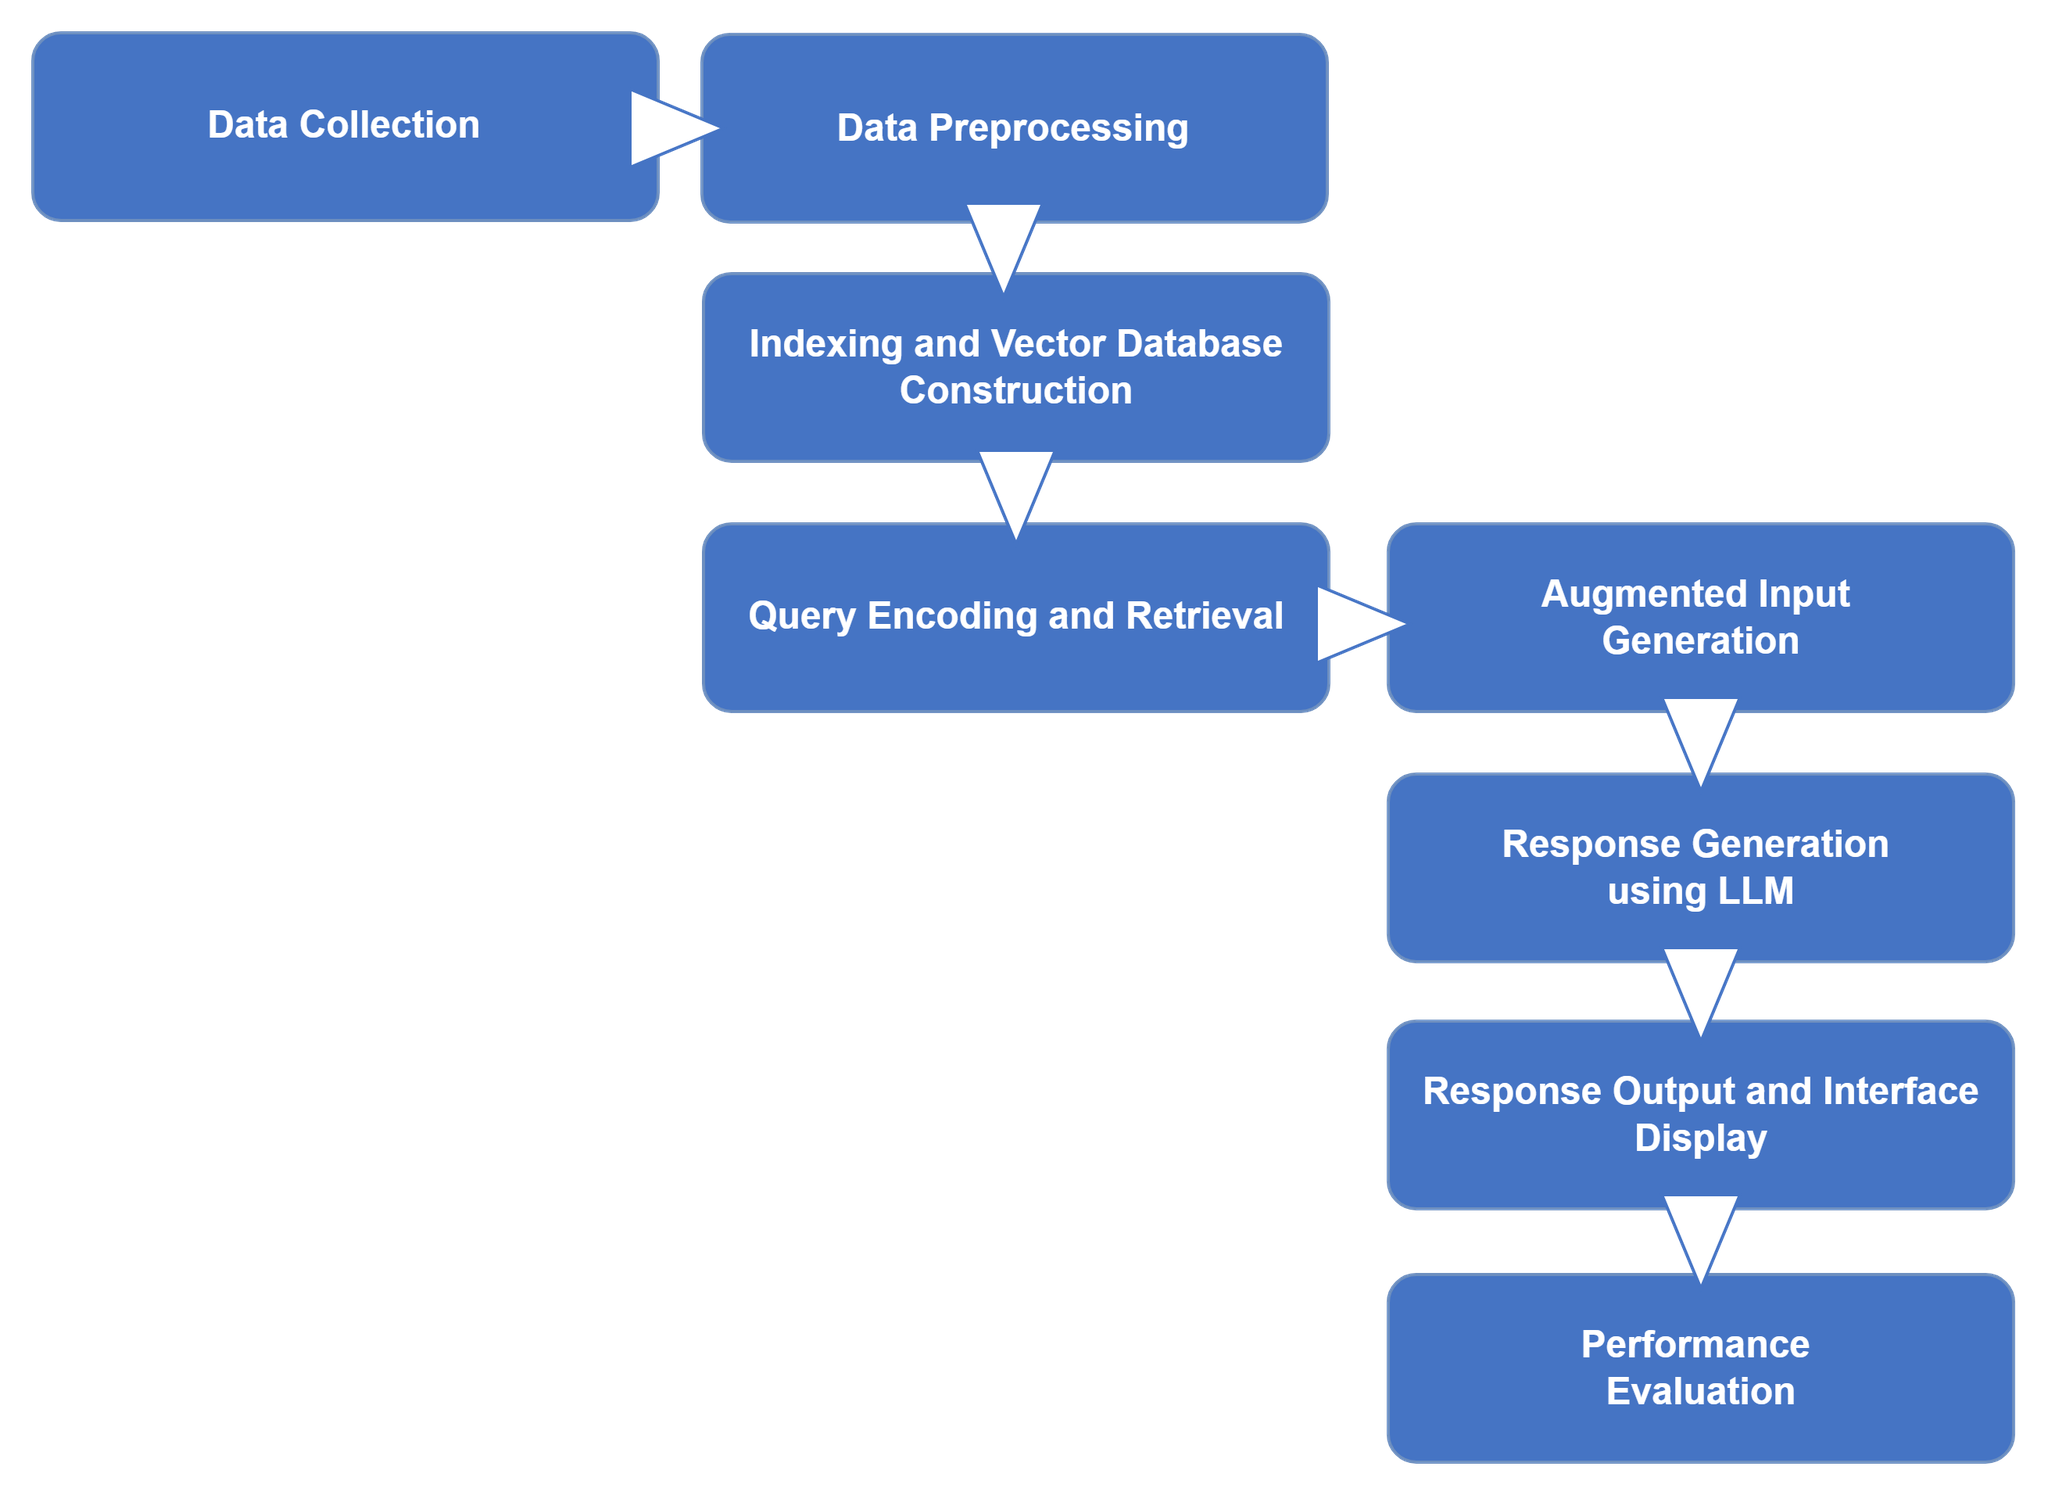
\includegraphics[width=0.7\textwidth]{figures/framework.png}
    \caption{Implementation of the Proposed Original Model}
\end{figure}

\section{Data Collection}
In this section, the researchers began with their proposal and coordination with CSPC Library and its staff, where the prototype was demonstrated to show how a RAG-powered chatbot could improve thesis discovery beyond exact-keyword search by enabling topic-oriented, semantically grounded retrieval within the library’s own repository. In the demonstration, the project’s institutional value was emphasized in accelerating literature searches, increasing access to relevant local theses, and supporting academic guidance, following the researchers' formal request to obtain one hundred undergraduate thesis PDFs from various College departments of CSPC to use as the main corpus of the RAG chatbot application.

\begin{figure}[h]
    \centering
    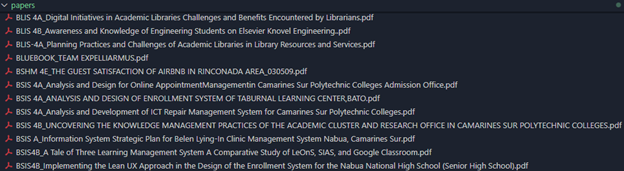
\includegraphics[width=0.7\textwidth]{figures/tsis_docs.png}
    \caption{CSPC Undergraduate Thesis Documents}
\end{figure}

Upon agreement on project scope, data handling practices, and local/on-premise deployment, library personnel granted the researchers to gain access to the digital copies of undergraduate thesis papers. The dataset was acknowledged and queued for the development phase following the proposed model pipelines’ process.

\subsection{Data Preprocessing}
This section commenced the systematic ingestion of the acquired thesis PDFs into the processing pipeline. Utilizing a custom script, the system recursively scanned the designated data folder housing more than 100 undergraduate thesis documents, ensuring all relevant files were accessed regardless of folder organization. Each PDF was processed page-by-page using the PyPDFLoader, extracting raw textual content alongside essential metadata such as source file paths and page numbers. This granular extraction maintained the academic formatting and pagination critical for preserving context, citations, and facilitating precise retrieval during later stages.

\begin{figure}[h]
    \centering
    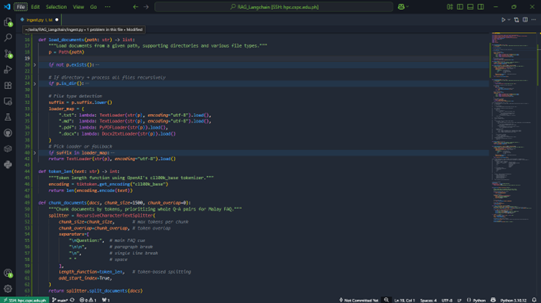
\includegraphics[width=0.7\textwidth]{figures/dtprprcss.png}
    \caption{Data Preprocessing inside the code editor}
\end{figure}

Extracted texts were segmented with a token-aware strategy (RecursiveCharacterTextSplitter), producing semantically coherent chunks sized to the LLM context window and guided by structural delimiters such as paragraph breaks and headings. Each chunk retained source, page, and positional offsets to support traceability and user navigation. The preprocessing yielded clean, contextually rich text segments ready for vectorization and indexing in the subsequent pipeline stage.    

\subsection{Indexing and Vector Database Construction}
The indexing phase transformed the preprocessed text chunks into a searchable knowledge base optimized for semantic retrieval within the RAG pipeline. This critical stage bridged the gap between raw textual content and the intelligent query-response capabilities that would define the chatbot's effectiveness in academic literature discovery.

\begin{figure}[h]
    \centering
    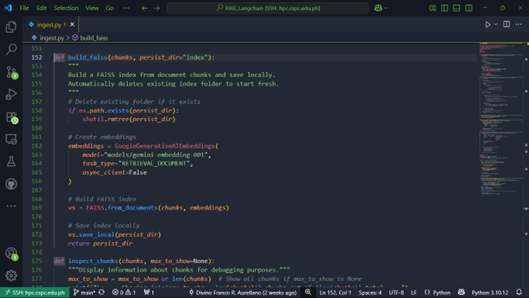
\includegraphics[width=0.7\textwidth]{figures/indfaiss.png}
    \caption{Indexing and Vector Database Construction}
\end{figure}

Each text chunk underwent embedding generation through the GoogleGenerativeAIEmbeddings model, which converted the semantic meaning of academic content into dense numerical vectors. This embedding process captured nuanced relationships between concepts, methodologies, and findings across the diverse corpus of CSPC thesis documents. The resulting vectors preserved both explicit textual information and implicit contextual relationships, enabling the system to understand queries about similar research topics, methodological approaches, or theoretical frameworks even when exact keywords differed. Following embedding generation, the vector representations were systematically indexed and stored within FAISS, a specialized library engineered for high-performance similarity search operations on dense vectors. The database construction process organized vectors using efficient indexing algorithms that would later enable rapid retrieval of contextually relevant thesis segments. Metadata preservation ensured that each vector maintained its connection to source documents, page numbers, and positional information, creating a comprehensive mapping between semantic concepts and their original academic contexts. This FAISS-based indexing architecture formed the retrieval foundation that would allow users to discover relevant thesis content through natural language queries, moving beyond traditional keyword matching to genuine semantic understanding of academic literature.


\subsection{Query Encoding and Retrieval}
The query processing stage represented the critical juncture where user intent transformed into actionable semantic search within the RAG chatbot system. This phase determined whether students and researchers would successfully locate relevant thesis content or encounter the frustrating "no results found" experience that plagued traditional keyword-based library systems.

\begin{figure}[h]
    \centering
    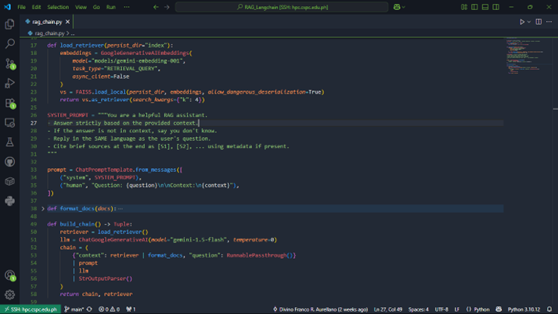
\includegraphics[width=0.7\textwidth]{figures/qandcntxtret.png}
    \caption{Question and Context Retrieval}
\end{figure}

When users submitted natural language queries such as "What research has been done on machine learning applications in healthcare?" or "Show me theses about sustainable energy solutions," the system initiated a sophisticated encoding process that mirrored the document preprocessing methodology. The user's question underwent vectorization using the identical GoogleGenerativeAIEmbeddings model employed during the indexing phase, ensuring semantic consistency between query representation and document storage. This encoding process transformed colloquial academic inquiries into dense numerical vectors that captured not just keywords but the conceptual intent and contextual nuances embedded within the user's research interests.

The retrieval mechanism leveraged the FAISS index infrastructure to execute high-speed similarity comparisons between the encoded query vector and the comprehensive collection of stored thesis document vectors. Using cosine similarity algorithms, the system calculated semantic distances to identify document chunks that most closely aligned with the user's informational needs. The top-K most relevant chunks—typically configured to retrieve four highly pertinent segments—were systematically selected and prepared for downstream processing. This retrieval approach transcended simple keyword matching, enabling the discovery of academically relevant content even when users employed different terminology, conceptual frameworks, or research perspectives than those found in the original thesis documents. The retrieved chunks formed the contextual foundation that would guide the language model's response generation, ensuring that chatbot answers remained grounded in actual CSPC thesis content rather than general knowledge or potential hallucinations.


\section{Augmented Input Generation}
The augmented input generation phase served as the crucial bridge between retrieved thesis content and intelligent response formulation, where raw document chunks evolved into contextually enriched prompts capable of guiding accurate academic discourse. Following successful retrieval of the top-K relevant thesis segments, the system executed a sophisticated concatenation process that preserved both content integrity and source attribution. Each retrieved document chunk underwent formatting that maintained its semantic value while incorporating lightweight citation markers such as "[S1 thesis_title.pdf p.15]" to ensure academic provenance remained traceable throughout the response generation process. This formatting approach created a unified context string that seamlessly wove together diverse thesis excerpts, methodological discussions, and research findings into a coherent knowledge foundation.

\begin{figure}[h]
    \centering
    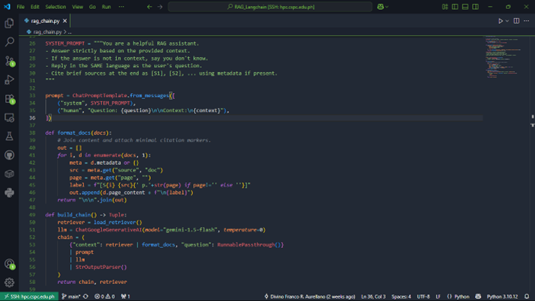
\includegraphics[width=0.7\textwidth]{figures/augInGen.png}
    \caption{Augmented Input Generation}
\end{figure}

The augmented prompt construction represented the culmination of the retrieval pipeline, where user queries and retrieved contexts merged into comprehensive input structures designed to optimize LLM performance within academic constraints. The system employed structured prompt templates to orchestrate a dual-component input framework consisting of system-level instructions that established academic rigor expectations and human-readable messages that combined the original user question with the formatted context string. This architectural approach ensured that the language model would receive explicit guidance to ground responses exclusively in provided thesis content while maintaining proper source citation practices. The pipeline incorporated practical safeguards, including token limit monitoring to prevent context overflow, intelligent truncation strategies for extensive retrievals, and explicit "no context available" indicators when insufficient relevant material existed, thereby maintaining input quality and preventing downstream processing issues.

\subsection{Response Generation}

The response generation stage represented the culmination of the RAG pipeline, where gemini-1.5-flash transformed augmented academic context into coherent, factually grounded answers that addressed user research inquiries. At this critical juncture, the language model processed the carefully constructed prompt containing both the original user question and the retrieved thesis content, leveraging its advanced reasoning capabilities to synthesize information from multiple academic sources into comprehensive responses. The system configured gemini-2.5-flash with temperature=0 to ensure deterministic output generation, eliminating randomness in responses and providing consistent answers when identical queries were posed. This deterministic approach proved essential for academic applications where reliability and reproducibility were paramount concerns for CSPC Library users seeking dependable research assistance.

\begin{figure}[h]
    \centering
    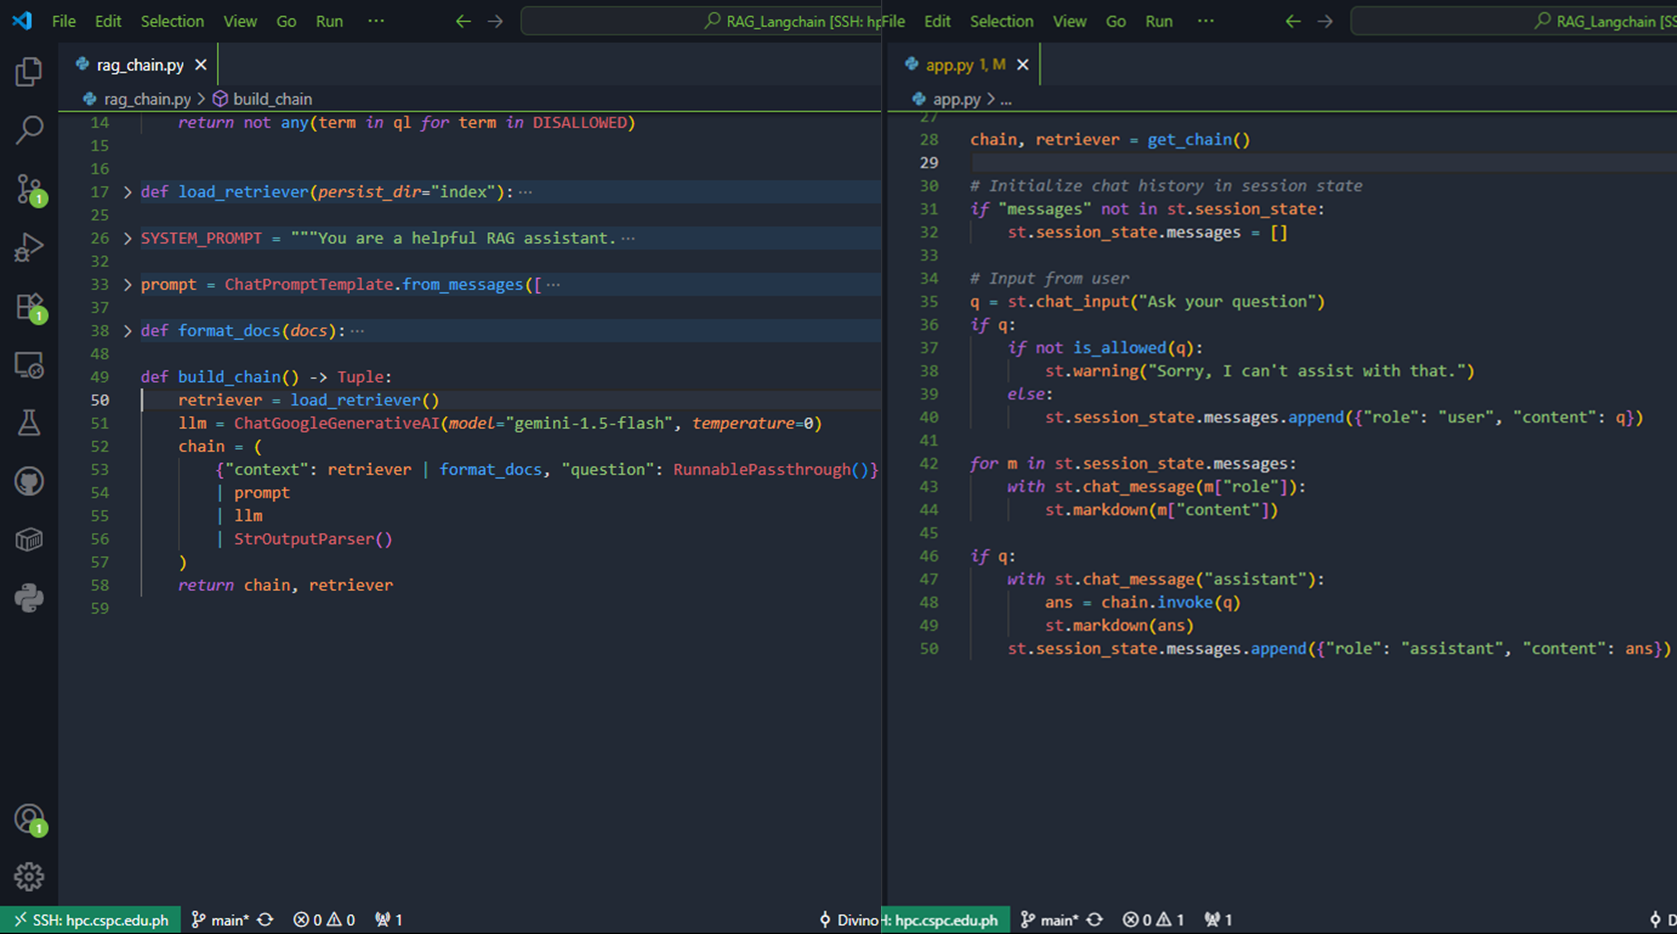
\includegraphics[width=0.7\textwidth]{figures/resgen.png}
    \caption{Response Generation}
\end{figure}   

The generation process operated through token-by-token prediction, where gemini-2.5-flash conditioned each response element on both the explicit system instructions and the augmented context, ensuring that generated content remained faithful to the retrieved thesis material rather than relying solely on pre-training knowledge. The model's reinforcement learning enhancements enabled sophisticated reasoning patterns that could identify relationships between different thesis segments, synthesize findings across multiple documents, and present information in academically appropriate formats. Following generation completion, the raw model output underwent parsing to yield clean text responses suitable for display within the chatbot interface. Despite the RAG framework's significant reduction in hallucination risks, the system maintained awareness that occasional inaccuracies could still occur when context was ambiguous or insufficient, necessitating user validation of critical research findings and encouraging cross-referencing with original source materials for comprehensive academic work.

\section{Response Output and Interface Display}

The final stage of user interaction materialized through a carefully designed Streamlit-based interface that transformed complex RAG processing into an intuitive conversational experience for CSPC Library users. When students and researchers submitted queries through the chat input interface, the system initiated a multi-layered safety and processing protocol that ensured both user protection and response quality. The application first executed content filtering mechanisms to verify query appropriateness before recording user messages in the session state, maintaining conversation continuity while preventing potentially harmful or inappropriate requests from reaching the underlying language model. This safety-first approach reflected the academic context where responsible AI deployment was essential for maintaining institutional standards and user trust.

\begin{figure}[h]
    \centering
    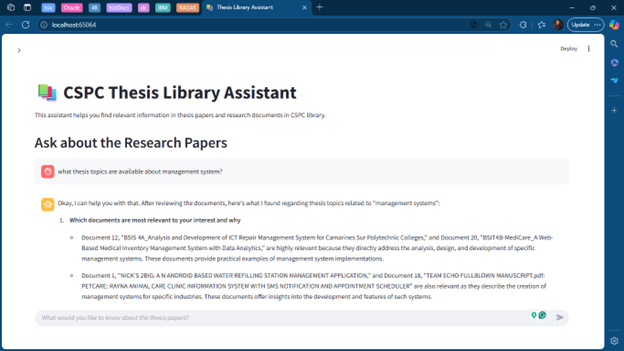
\includegraphics[width=0.7\textwidth]{figures/streamlit.png}
    \caption{Streamlit Interface Display}
\end{figure}

Following successful query validation, the cached RAG chain executed the complete retrieval and generation workflow through a single invoke call that orchestrated document retrieval, context formatting, and LLM response generation in a seamless pipeline. The interface architecture preserved conversation history by maintaining all user and assistant interactions within the session state, enabling users to reference previous exchanges and build upon earlier research discussions throughout extended library sessions. Generated responses appeared as rendered Markdown content that supported academic formatting including citations, lists, and structured text presentation, while the lightweight citation markers embedded within retrieved context enabled users to trace answers back to specific thesis documents and page references. When queries violated safety parameters, the system displayed clear Streamlit warnings instead of processing requests, maintaining transparent communication about system limitations. The synchronous processing approach with deterministic temperature settings ensured consistent response quality and eliminated unpredictable variations that could undermine user confidence in the academic research tool, while the persistent conversation interface encouraged iterative inquiry and deeper exploration of CSPC's thesis repository through natural dialogue.

\section{Model Evaluation}
In this section, the RAG-based chatbot system for the CSPC Library was evaluated utilizing four critical metrics: Answer Relevancy, Context Precision, Context Recall, and Faithfulness. These metrics provide a multidimensional perspective on the performance of the literature retrieval system, ensuring robust analysis in both information quality and reliability. The evaluation framework and explanations are patterned after established academic standards as demonstrated in the reference thesis.

\section{Result}
This section presents the findings through tables, figures, and subsequent discussion. Prior to evaluation, a systematic data processing pipeline was applied: 200+ undergraduate thesis PDFs from the CSPC Library were processed into segmented meaningful text chunks, and embedded using Hugging Face's Embeddings. These chunks were indexed in FAISS for efficient semantic retrieval, enabling the RAG chatbot to generate contextually relevant and factually grounded responses for user queries. This process ensured that the evaluation was conducted on high-quality, well-structured academic data.

\begin{table}[H]
    \centering
    \caption{RAG System Evaluation Metrics}
    \begin{tabular}{|l|c|}
        \hline
        \textbf{Metric} & \textbf{Average Score} \\
        \hline
        Answer Relevancy   & 0.737 \\
        Context Precision  & 0.818 \\
        Context Recall     & 0.721 \\
        Faithfulness       & 0.585 \\
        \hline
    \end{tabular}
\end{table}

\noindent The table above provides a concise summary of the RAG system’s evaluation metrics, offering a clear view of its performance in literature search and thesis retrieval tasks. Each metric captures a distinct aspect of the system’s effectiveness:

\begin{enumerate}
\item \textbf{Answer Relevancy (0.737):} This metric reflects how well the system’s responses address user queries. A score of 0.737 indicates that the chatbot generally provides answers that are relevant and useful, supporting users in finding the information they seek.
\item \textbf{Context Precision (0.818):} Context precision measures the proportion of retrieved text chunks that are actually relevant to the query. With a high score of 0.818, the system demonstrates strong ability to filter out irrelevant information, ensuring that users receive focused and meaningful content.
\item \textbf{Context Recall (0.721):} This metric assesses the system’s ability to retrieve all relevant information needed to answer a query. A score of 0.721 suggests that the chatbot successfully gathers most of the necessary supporting content, though there is still room for improvement in capturing every relevant detail.
\item \textbf{Faithfulness (0.585):} Reflects how accurately the chatbot's generated responses were supported by the source documents. While lower than other metrics, this value highlights a key area for improvement, emphasizing the challenge of maintaining strict factual consistency in generative retrieval systems.
\end{enumerate}

\noindent These metrics offer a comprehensive view of the system’s effectiveness. High answer relevancy and context precision demonstrate the chatbot’s practicality and efficiency in delivering relevant results, while context recall and faithfulness underscore the system’s coverage and reliability. Faithfulness, in particular, remains an ongoing focus for enhancement, aligning with current research advances in AI literature retrieval. These metrics collectively form the foundation for interpreting, tuning, and extending the RAG chatbot’s capabilities within the CSPC Library environment.

\begin{figure}[h]
    \centering
    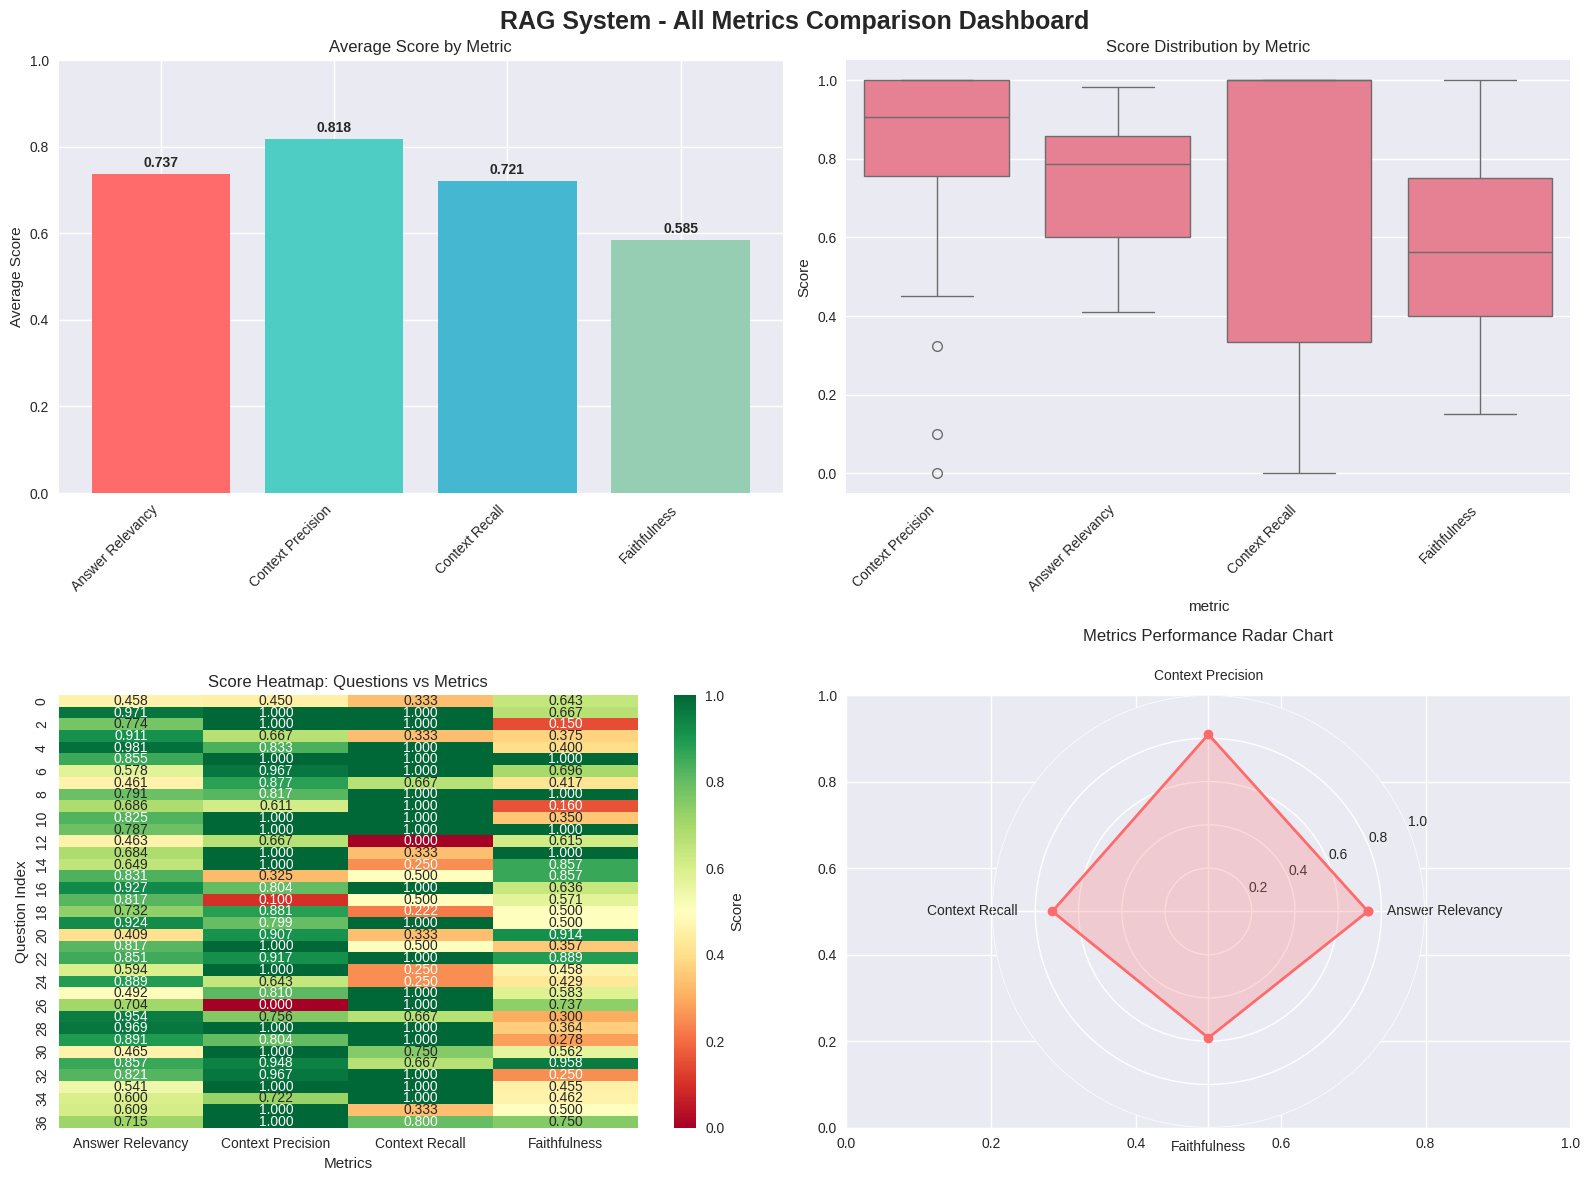
\includegraphics[width=0.7\textwidth]{figures/overall_out.png}
    \caption{RAG System - Metrics Dashboard}
\end{figure}

\section*{RAG System - Metrics Dashboard}
The dashboard presented herein serves as an integrated visualization tool for evaluating the RAG system’s performance across four core metrics: Answer Relevancy, Context Precision, Context Recall, and Faithfulness. Each chart within the dashboard offers unique insights into different aspects of system behavior in the context of literature search and thesis retrieval.
\noindent The bar chart illustrates the average score attained for each metric. Notably, Context Precision achieves the highest average (0.818), followed by Answer Relevancy (0.737), Context Recall (0.721), and Faithfulness (0.585). This ordering highlights the system’s exceptional ability to retrieve relevant information, moderate competence in delivering complete and relevant answers, and a comparative need for improvement in grounding generated responses strictly within the source material.
\noindent The box plot details the score distribution across metrics, emphasizing both consistency and spread. Metrics such as Context Precision and Answer Relevancy display less variance and higher minimum scores, indicating stable system performance. In contrast, Context Recall and Faithfulness exhibit a broader range, evidencing occasional lapses in comprehensive retrieval and accurate grounding.
\noindent The heatmap provides a granular view by displaying metric scores for individual questions. Darker shades correspond to higher scores, meaning better performance for both retrieval and generation on those specific queries. The heatmap reveals that while the chatbot excels on many questions, there is still inconsistency—some queries show lower faithfulness or recall, suggesting targets for further system refinement.
\noindent The radar chart synthesizes the metric scores into a single shape, depicting the RAG system’s overall performance profile at a glance. The profile is robust in Context Precision and Answer Relevancy, slightly reduced in Context Recall, and tapers at Faithfulness. This visualization makes clear where the system currently excels and where enhancements should be prioritized.

These visualizations collectively deliver a comprehensive, multi-faceted overview of the RAG chatbot’s strengths and areas for further enhancement. The visualizations reveal the system’s strong retrieval precision and relevancy, adequate recall, and opportunities for improvement regarding faithfulness to source documents. These insights guide ongoing refinements to optimize the chatbot for reliable, accurate, and comprehensive academic information retrieval.

%=======================================================%
%%%%% Do not delete this part %%%%%%
\clearpage

\printbibliography[heading=subbibintoc, title={\centering Notes}]
\end{refsection}
    
\chapter{Summary of Findings, Conclusion and Recommendations}
\begin{refsection}
In this chapter, the RAG Chatbot for Efficient Literature Search and Thesis Retrieval in the CSPC Library is discussed. The information presented in this chapter is entirely based on the data that were gathered during the data collection and system development processes. The purpose of this chapter is to provide a summary of the results, conclusions, and research recommendations for additional study.

\section{Summary}
The RAG-based chatbot for efficient literature search and thesis retrieval in the CSPC Library was successfully developed and evaluated as part of this project. The system integrates Retrieval-Augmented Generation (RAG) techniques with vector embeddings and the Google Gemini large language model to enable semantic search, providing more accurate and contextually relevant results compared to traditional keyword-based search methods. The development process included modules for document ingestion, preprocessing, indexing, and storage, which ensured that the thesis repository was machine-readable and well-structured. The user interface was designed to be intuitive and user-friendly, allowing users to easily interact with the chatbot and retrieve relevant theses based on their queries. The system was evaluated through a series of tests, including accuracy, response time, which demonstrated its effectiveness in improving literature search and thesis retrieval processes.

\section{Findings}
Based on the results and discussions presented in Chapter 4, the following findings were derived from the
\begin{enumerate}
    \item Successful Document Ingestion and Preprocessing
The system effectively ingested and preprocessed all available thesis PDFs collected from the CSPC Library. Metadata such as page numbers, file names, and headings were preserved, ensuring academic integrity and accurate referencing of documents. This guaranteed that the repository was machine-readable and ready for retrieval operations.
    \item Efficient Indexing and Storage
The use of vector embeddings and a vector database allowed for efficient indexing and storage of the preprocessed thesis documents. This enabled fast and accurate retrieval of relevant documents based on semantic similarity, significantly improving the search experience for users.
    \item Improved Query Handling and Response Generation
The integration of the Google Gemini large language model with the RAG framework allowed for effective query handling and response generation. The chatbot was able to understand user queries in natural language and provide contextually relevant responses, enhancing the overall user experience.
    \item User-Friendly Interface
The user interface was designed to be intuitive and easy to navigate, allowing users to interact with the chatbot seamlessly. Users could input their queries and receive responses without requiring technical knowledge, making the system accessible to a wide range of users.
    \item Positive Evaluation Results
\end{enumerate}

\section{Conclusion}
Based on the findings, the researchers came up with the following conclusion:
\begin{enumerate}
    \item The RAG-based chatbot for efficient literature search and thesis retrieval in the CSPC Library was successfully developed and implemented, demonstrating the feasibility of using advanced AI techniques to enhance academic research processes.
    \item The system effectively improved the accuracy and relevance of search results compared to traditional keyword-based search methods, providing users with more contextually appropriate theses based on their queries.
    \item The integration of vector embeddings and the Google Gemini large language model proved to be effective in handling natural language queries and generating relevant responses, showcasing the potential of combining retrieval and generation techniques in information retrieval systems.
    \item The user-friendly interface contributed to a positive user experience, making it easy for users to interact with the chatbot and access relevant academic resources without requiring technical expertise.


    % \item The RAG-based chatbot demonstrated strong potential for enhancing academic research workflows, providing a valuable tool for students and researchers at CSPC.
    % \item The successful implementation of the RAG framework in this project highlights the importance of leveraging advanced AI techniques to address challenges in information retrieval and academic research.
\end{enumerate}
%=======================================================%
%%%%% Do not delete this part %%%%%%
\clearpage

\printbibliography[heading=subbibintoc, title={\centering Notes}]
\end{refsection}

    \makeBibliography
    % 
% The environment used here (theappendices) is a wrapper for the basic appendices environment which changes the appearance of the title page and the structure and appearance of the appendices in the table of contents and PDF bookmarks. The original functionality can be restored by simply removing the 'the' from the \begin{} and \end{} statements below.

\begin{theappendices}

\chapter{Language Editing Certification}
\centering

This is to certify that the undersigned has reviewed and went through all the pages of the Bachelor of Science in Computer Science thesis manuscript titled \\

\textbf{"ENTER YOUR TITLE HERE"} \\


of \textbf{AuthorName1}, \textbf{AuthorName2}, \textbf{AuthorName3}, as against the set of structural rules that govern research writing in accord with the composition of sentences, phrases, and words in the English language.
 \newline \newline \newline \\

\noindent \textbf{JUAN DE LA CRUZ} \\
\textit{Language Editor} \\

Date:\_\_\_\_\_\_\_\_\_\_\_\_\_\_\_\_\_\_\_\_\_\_\_


\chapter{Secretary's Certification}
\centering

This is to certify that the undersigned has provided accurate recommendations, suggestions, and comments unanimously agreed and approved by the panel of examiners during the oral examination of the thesis titled \\ \textbf{"ENTER YOUR TITLE HERE"} \\  prepared and submitted by \textbf{AuthorName1}, \textbf{AuthorName2}, \textbf{AuthorName3}, and that the same have not been amended, modified or obliterated. \newline \newline \newline \\



\textbf{MS. MARIA DAISY R. BELARDO} \\
\textit{Secretary} \\


Date:\_\_\_\_\_\_\_\_\_\_\_\_\_\_\_\_\_\_\_\_\_\_\_

\chapter{JOINT AFFIDAVIT OF UNDERTAKING (Plagiarism)}

\centering

\textbf{JOINT AFFIDAVIT OF UNDERTAKING}


% IN WITNESS WHEREOF, I have hereunto set my name this ____ day of ___________ 202__ in
% ___________________________________, Philippines.
% SUBSCRIBED AND SWORN TO before me this ___ day of ________ at _______________, Philippines,
% affiants exhibiting to me their competent proofs of identity above stated.
% Doc. No. ___________:
% Page No.: __________:
% Book No.: __________:
% Series of 202_.


\end{theappendices}
    % % Vita should only be included for PhD candidates.

\begin{vita}

\begin{itemize}
    \item 
    
    \begin{figure}[ht]
        \centering
    	
\includegraphics[width=0.35\textwidth]{figures/person-icon.png}
    \end{figure}
    
    \textbf{Joseph Jessie S. Oñate} is a faculty member of the College of Computer Studies. He finished his Master of Science in Computer Science degree at Ateneo de Naga University. His research interests focused on Intelligent Systems, Algorithm and Complexity, Web Technologies, Computer Vision, and Graphics.
    
    \item 
    
    \begin{figure}[ht]
        \centering
    	
\includegraphics[width=0.35\textwidth]{figures/person-icon.png}
    \end{figure}
    
    \textbf{Joseph Jessie S. Oñate} is a faculty member of the College of Computer Studies. He finished his Master of Science in Computer Science degree at Ateneo de Naga University. His research interests focused on Intelligent Systems, Algorithm and Complexity, Web Technologies, Computer Vision, and Graphics.
    
    \item 
    
    \begin{figure}[ht]
        \centering
    	
\includegraphics[width=0.35\textwidth]{figures/person-icon.png}
    \end{figure}
    
    \textbf{Joseph Jessie S. Oñate} is a faculty member of the College of Computer Studies. He finished his Master of Science in Computer Science degree at Ateneo de Naga University. His research interests focused on Intelligent Systems, Algorithm and Complexity, Web Technologies, Computer Vision, and Graphics.
\end{itemize}

\end{vita}
\end{thesisbody}

\end{document}
